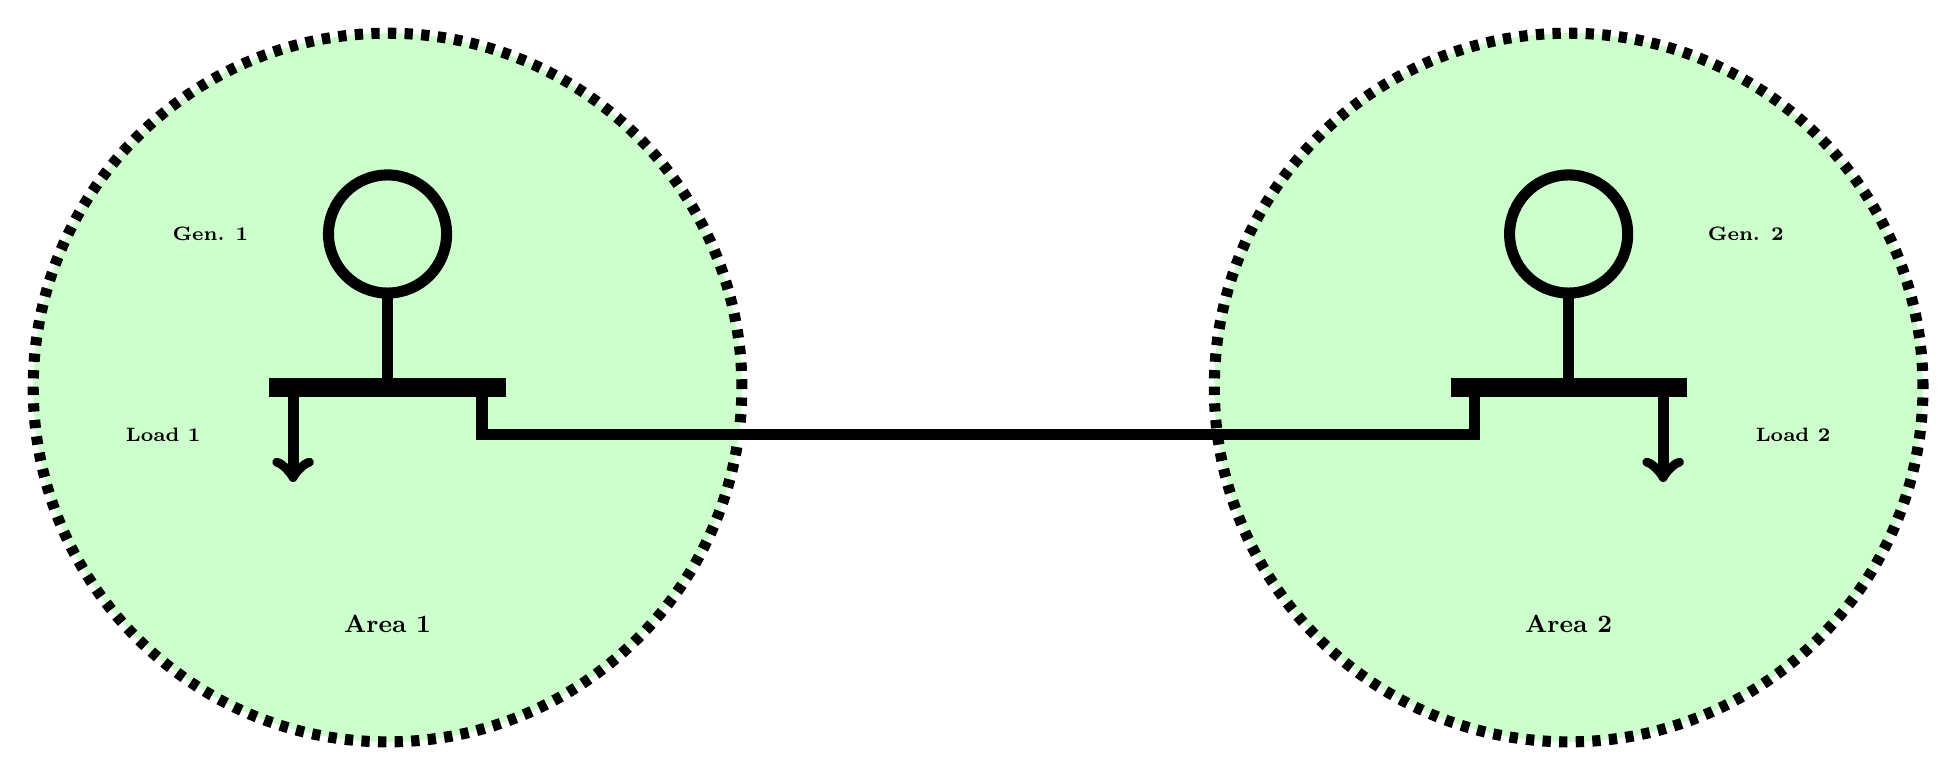
\begin{tikzpicture}
	
	% Area 1
	\draw [dashed, fill=green!20, line width=4pt] (3*0.5,0) circle (3*1.5cm);
		
	% Area 2
	\draw [dashed, fill=green!20, line width=4pt] (3*5.5,0) circle (3*1.5cm);
	
	% Area labels
	\node at (3*0.5,3*-1) {\small\textbf{Area 1}};
	\node at (3*5.5,3*-1) {\small\textbf{Area 2}};
	
	% Bus 1
	\draw [line width=7pt] (0,0) -- (3*1,0);
	\draw [line width=4pt] (3*0.5,0) -- (3*0.5,3*0.4);
	
	% Load 1
	\draw [->, line width=4pt] (3*0.1,0) -- (3*0.1,3*-0.4);
	\node at (3*-0.45,3*-0.2) {\scriptsize \textbf{Load 1}};
	
	% Gen 1
	\draw [line width=4pt] (3*0.5,3*0.65) circle (3*0.25cm);
	\node at (3*-0.25,3*0.65) {\scriptsize \textbf{Gen. 1}};
	
	% Bus 2
	\draw [line width=7pt] (3*5,0) -- (3*6,0);
	\draw [line width=4pt] (3*5.5,0) -- (3*5.5,3*0.4);
	
	% Load 2
	\draw [->, line width=4pt] (3*5.9,0) -- (3*5.9,3*-0.4);
	\node at (3*6.45,3*-0.2) {\scriptsize \textbf{Load 2}};
	
	% Gen 2
	\draw [line width=4pt] (3*5.5,3*0.65) circle (3*0.25cm);
	\node at (3*6.25,3*0.65) {\scriptsize \textbf{Gen. 2}};
	
	% Tie line 1 to 2
	\draw [line width=4pt] (3*0.9,0) -- (3*0.9,3*-0.2) -- (3*5.1,3*-0.2) -- (3*5.1,0);

\end{tikzpicture}
